\subsection{Feature Engineering}
In order to manage categorical data, it is essential to employ one-hot encoding to `type' feature. Other attributes seem to be usable because they can easily be used as inputs for the model. However, I need to do some data cleaning to make the data more suitable for our analysis. The first thing I did was to remove the `nameOrig' and `nameDest' columns because they are not useful for our analysis. The ‘isFlaggedFraud’ column is a simple indicator variable for whether the amount transferred in a given transaction exceeds the threshold of 200,000 - also must be removed. After derive the `step' field to `hour', the final dataset is shown in Figure 2.3.

\begin{figure}[H]
    \centering
    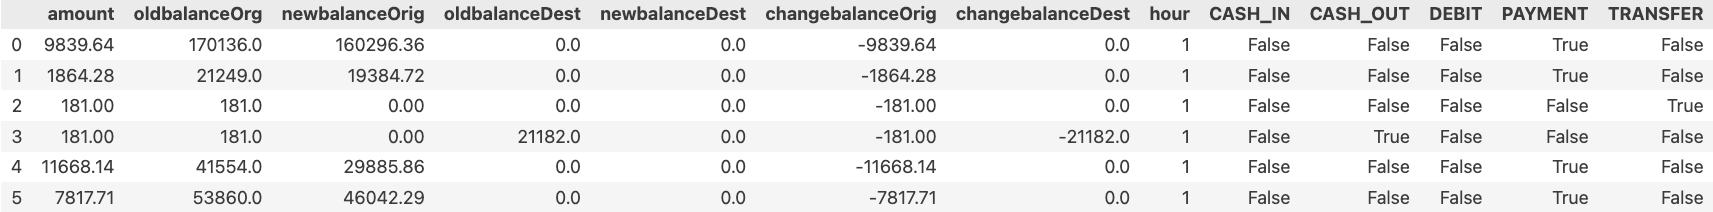
\includegraphics[width=\linewidth]{body/02_methodology/img/figure2.png}
    \caption{Final dataset}
\end{figure}
